\newcommand{\stepprefix}[1]{Step $#1$ - }

% Init

\begin{frame}{Parallel bijection - An example for $\Av{123}$ and $\Av{132}$}
    \begin{figure}
        \tikz{\draw [black, opacity=0] (0,0) rectangle (10,7.5);}
        \tikz [remember picture,overlay] \node at ([yshift=-.25cm,xshift=0cm]current page.center) {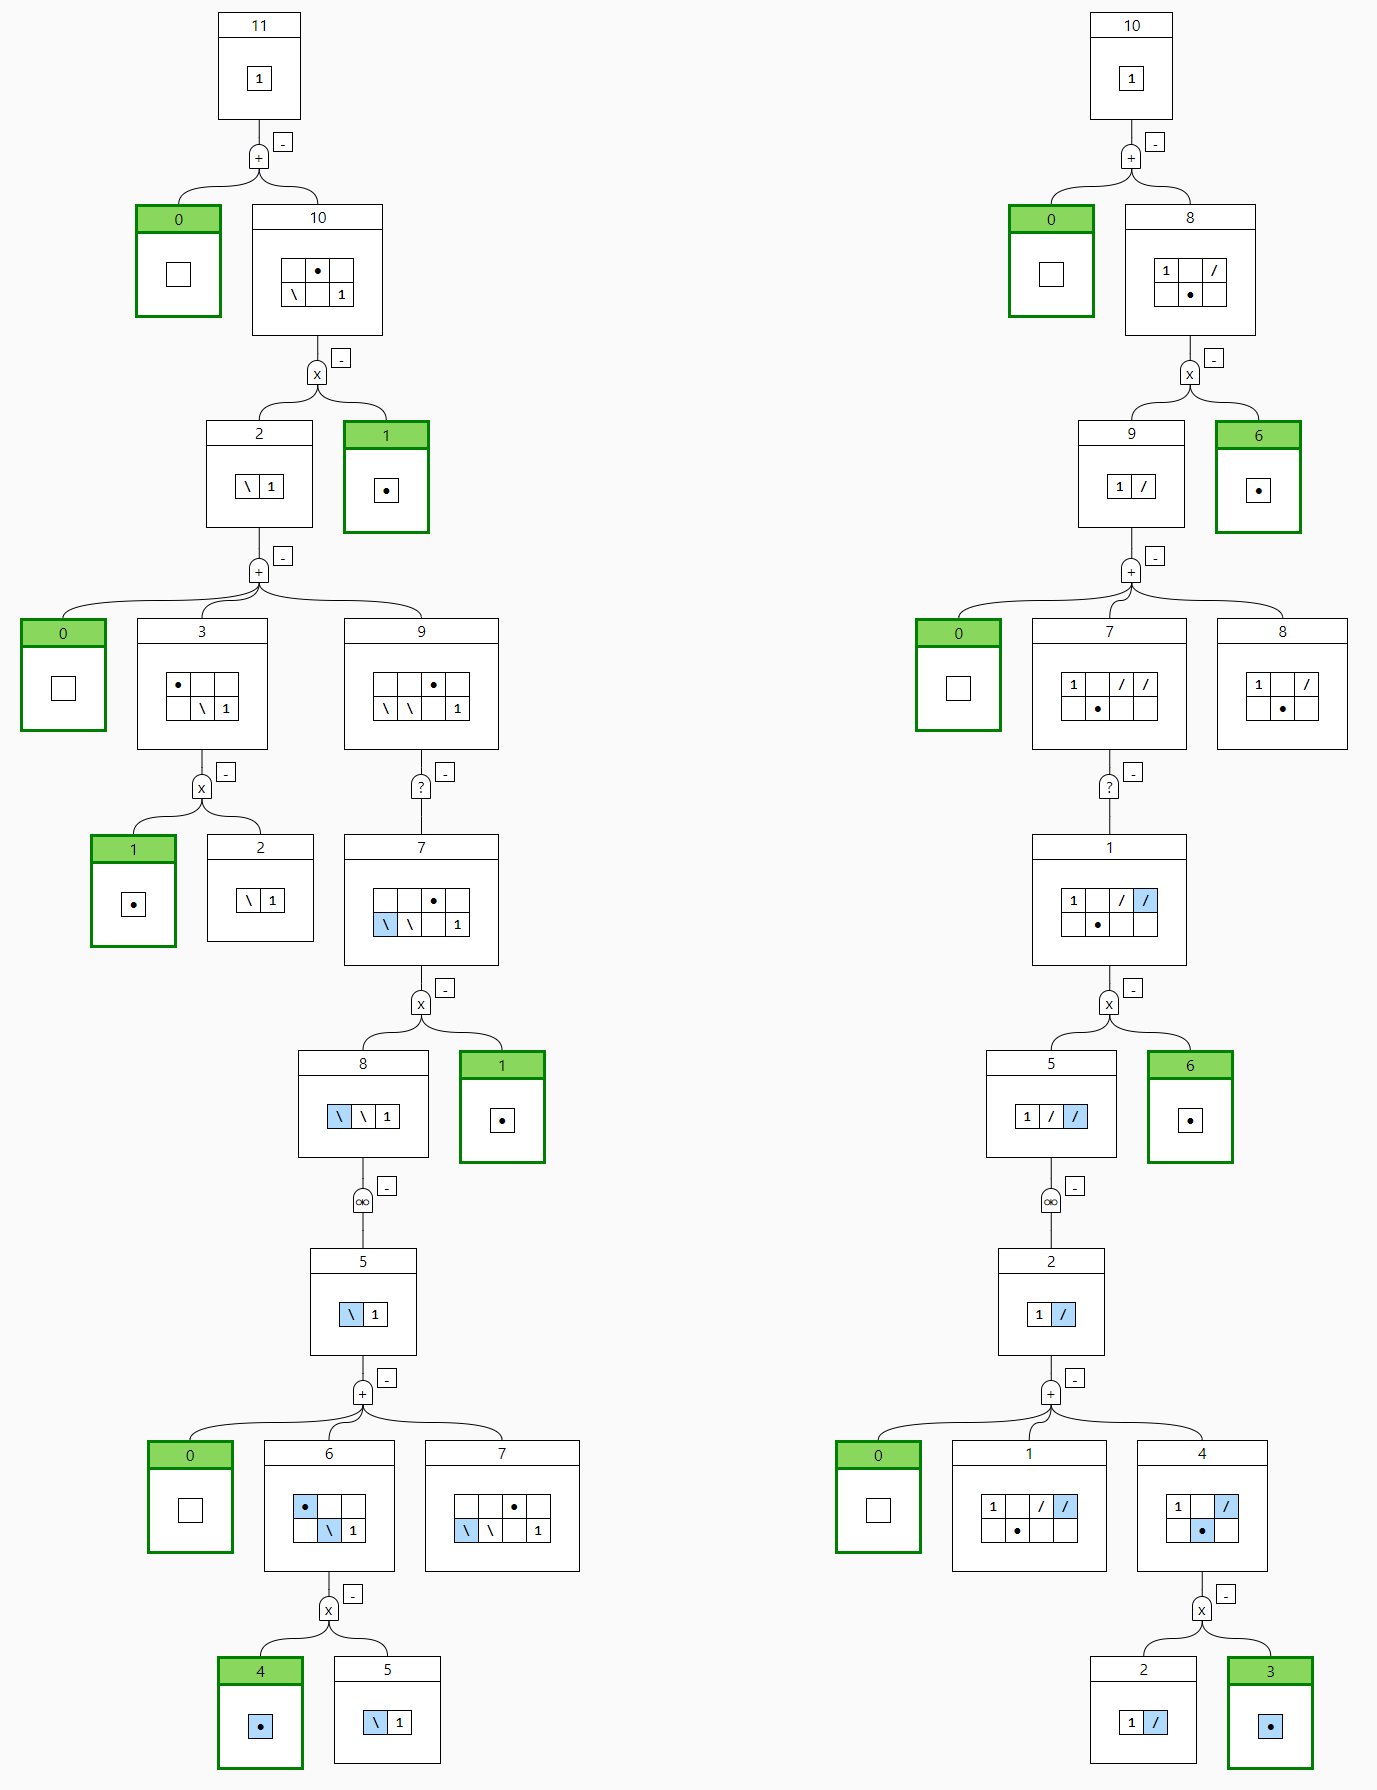
\includegraphics[scale=0.163]{graphics/123_132_specs.png}};
        \caption{Parallel specifications for $\Av{123}$ and $\Av{132}$.}
    \end{figure}
\end{frame}

% Forward steps

\begin{frame}{Parallel bijection - An example for $\Av{123}$ and $\Av{132}$}
    \begin{figure}
        \centering
        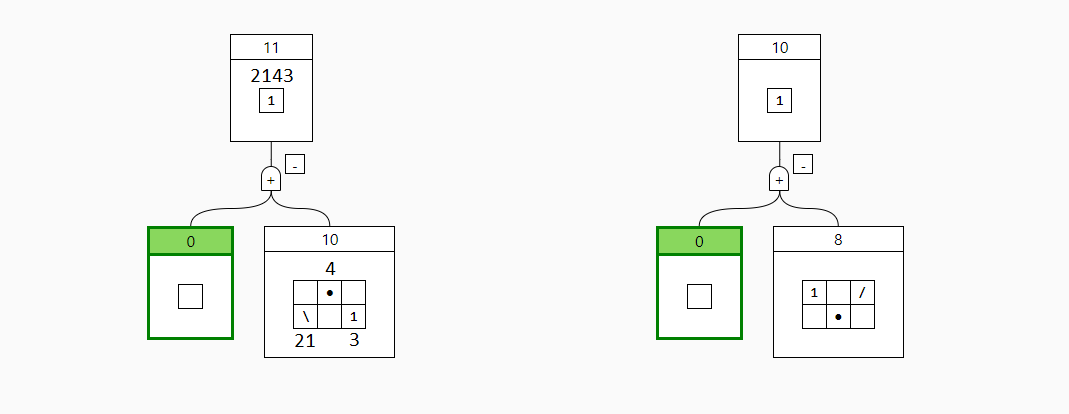
\includegraphics[scale=0.4]{graphics/step01.png}
        \caption{\stepprefix{1}Place topmost point of $2143$ in $\Av{123}$.}
    \end{figure}
\end{frame}

\begin{frame}{Parallel bijection - An example for $\Av{123}$ and $\Av{132}$}
    \begin{figure}
        \centering
        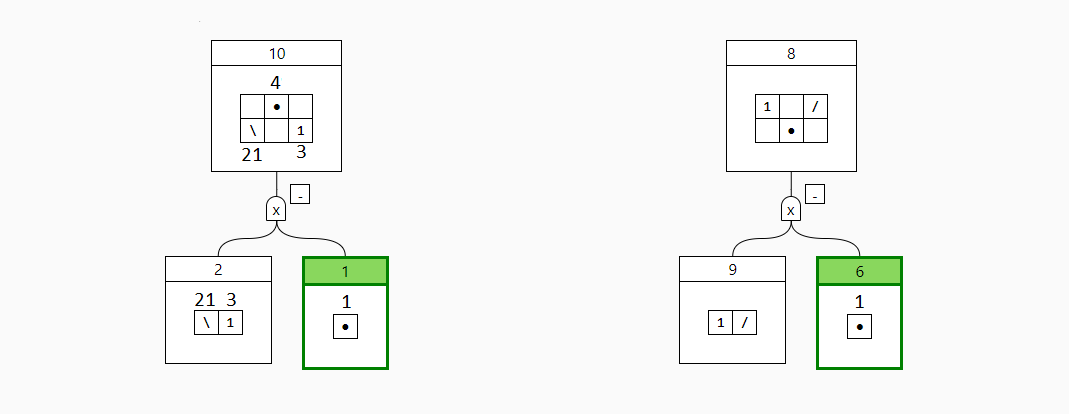
\includegraphics[scale=0.4]{graphics/step02.png}
        \caption{\stepprefix{2}Factor.}
    \end{figure}
\end{frame}


\begin{frame}{Parallel bijection - An example for $\Av{123}$ and $\Av{132}$}
    \begin{figure}
        \centering
        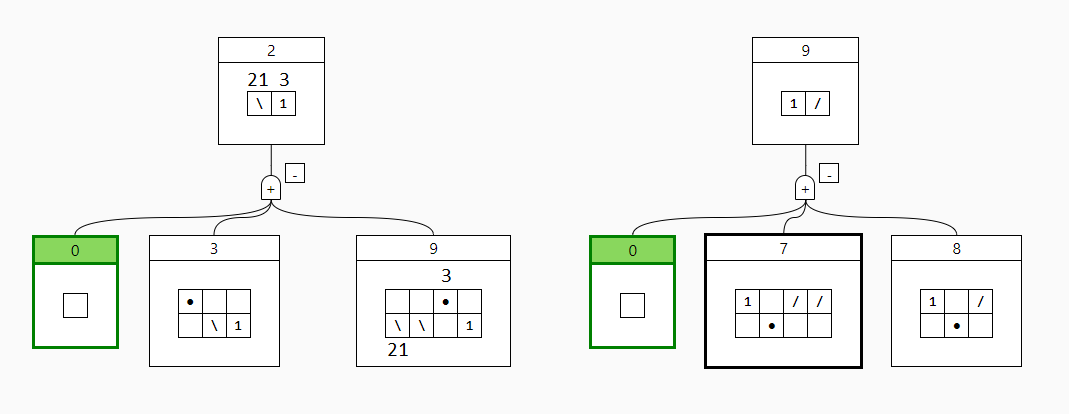
\includegraphics[scale=0.4]{graphics/step03.png}
        \caption{\stepprefix{3}Place topmost in row.}
    \end{figure}
\end{frame}

\begin{frame}{Parallel bijection - An example for $\Av{123}$ and $\Av{132}$}
    \begin{figure}
        \centering
        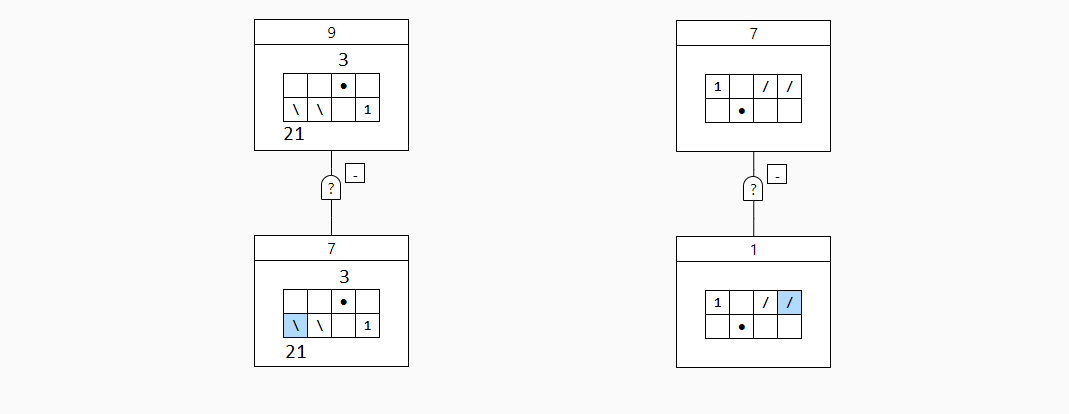
\includegraphics[scale=0.4]{graphics/step04.png}
        \caption{\stepprefix{4}Add assumption in $(0,0)$.}
    \end{figure}
\end{frame}

\begin{frame}{Parallel bijection - An example for $\Av{123}$ and $\Av{132}$}
    \begin{figure}
        \centering
        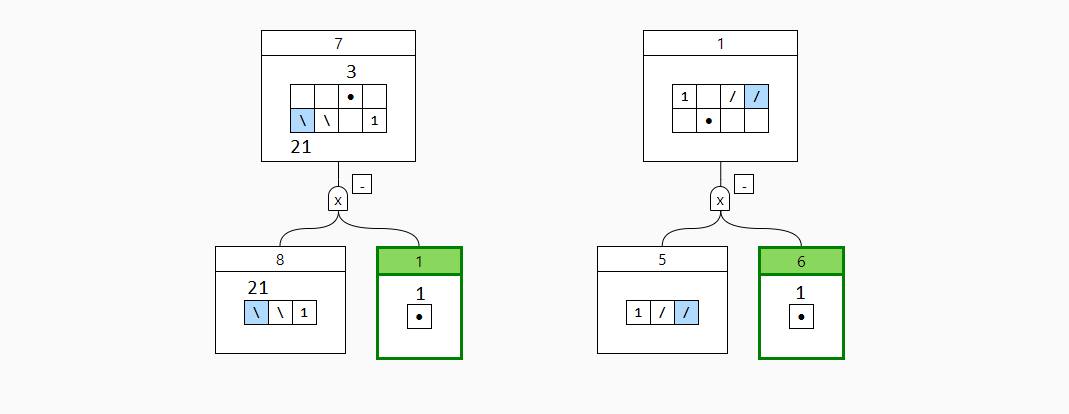
\includegraphics[scale=0.4]{graphics/step05.png}
        \caption{\stepprefix{5}Factor.}
    \end{figure}
\end{frame}


\begin{frame}{Parallel bijection - An example for $\Av{123}$ and $\Av{132}$}
    \begin{figure}
        \centering
        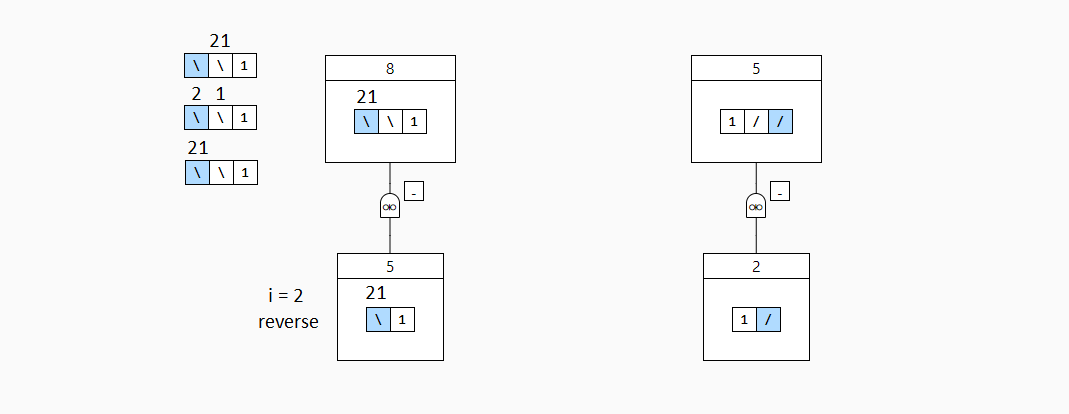
\includegraphics[scale=0.4]{graphics/step06.png}
        \caption{\stepprefix{6}Fuse columns $0$ and $1$.}
    \end{figure}
\end{frame}

\begin{frame}{Parallel bijection - An example for $\Av{123}$ and $\Av{132}$}
    \begin{figure}
        \centering
        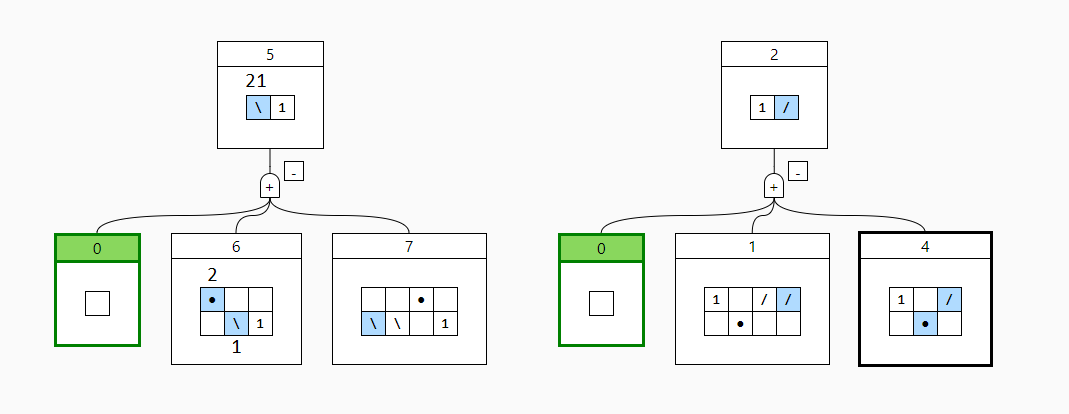
\includegraphics[scale=0.4]{graphics/step07.png}
        \caption{\stepprefix{7}Place topmost in row.}
    \end{figure}
\end{frame}

\begin{frame}{Parallel bijection - An example for $\Av{123}$ and $\Av{132}$}
    \begin{figure}
        \centering
        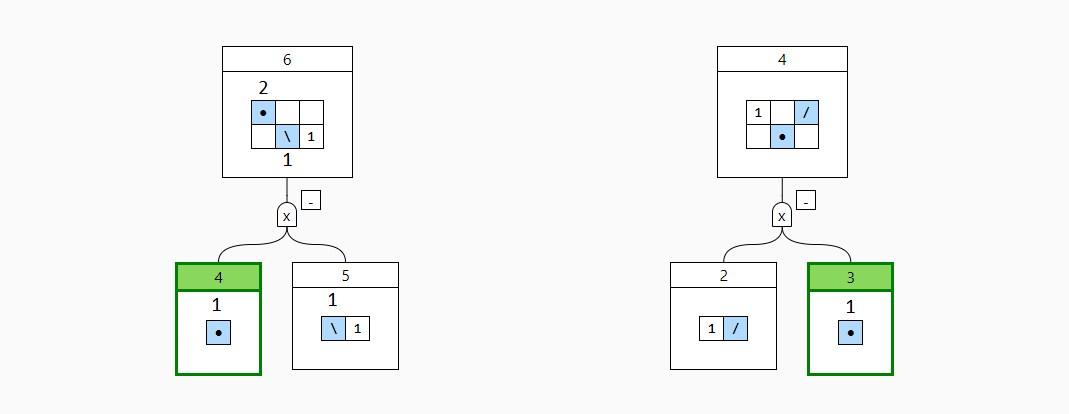
\includegraphics[scale=0.4]{graphics/step08.png}
        \caption{\stepprefix{8}Factor.}
    \end{figure}
\end{frame}

\begin{frame}{Parallel bijection - An example for $\Av{123}$ and $\Av{132}$}
    \begin{figure}
        \centering
        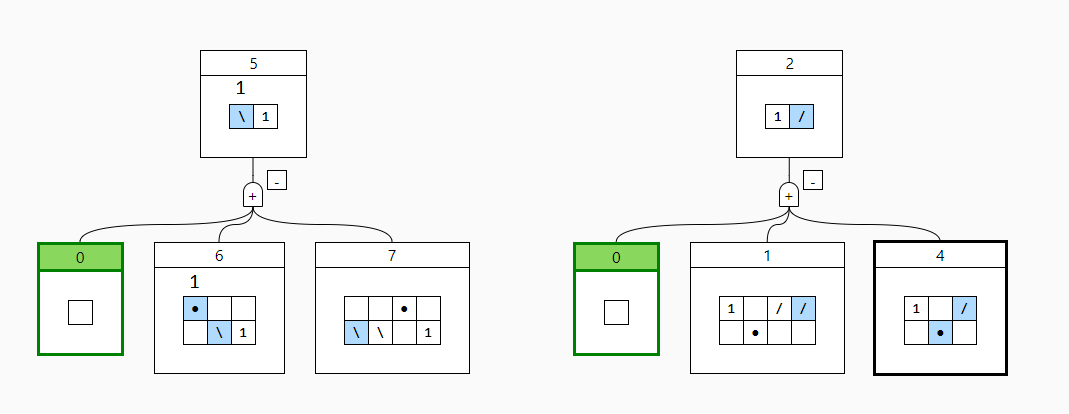
\includegraphics[scale=0.4]{graphics/step09.png}
        \caption{\stepprefix{9}Place topmost in row.}
    \end{figure}
\end{frame}

\begin{frame}{Parallel bijection - An example for $\Av{123}$ and $\Av{132}$}
    \begin{figure}
        \centering
        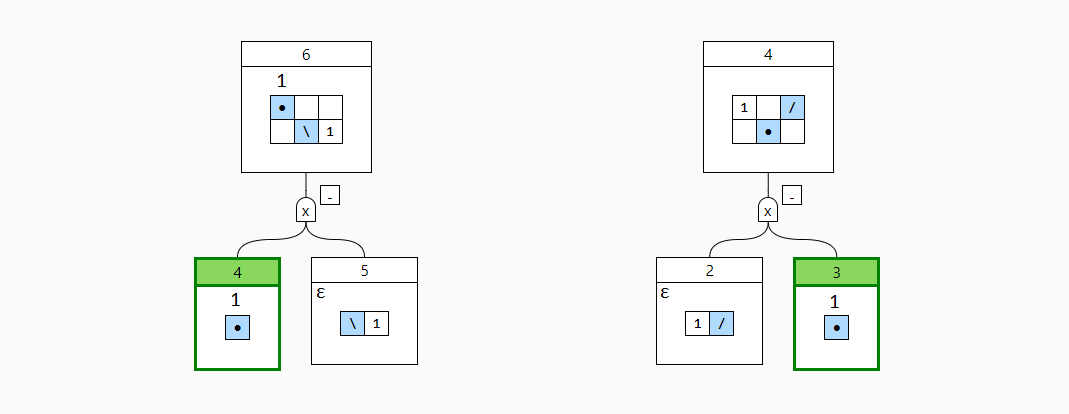
\includegraphics[scale=0.4]{graphics/step10.png}
        \caption{\stepprefix{10}Factor.}
    \end{figure}
\end{frame}

% Parse trees

\begin{frame}{Parallel bijection - An example for $\Av{123}$ and $\Av{132}$}
    %The parse tree we have created for $\Av{132}$.
    \begin{figure}
        \centering
        \tikz{\draw [black, opacity=0] (0,0) rectangle (10,7.5);}
        \only<1>{%
            \tikz [remember picture,overlay] \node at ([yshift=-.25cm,xshift=0cm]current page.center) {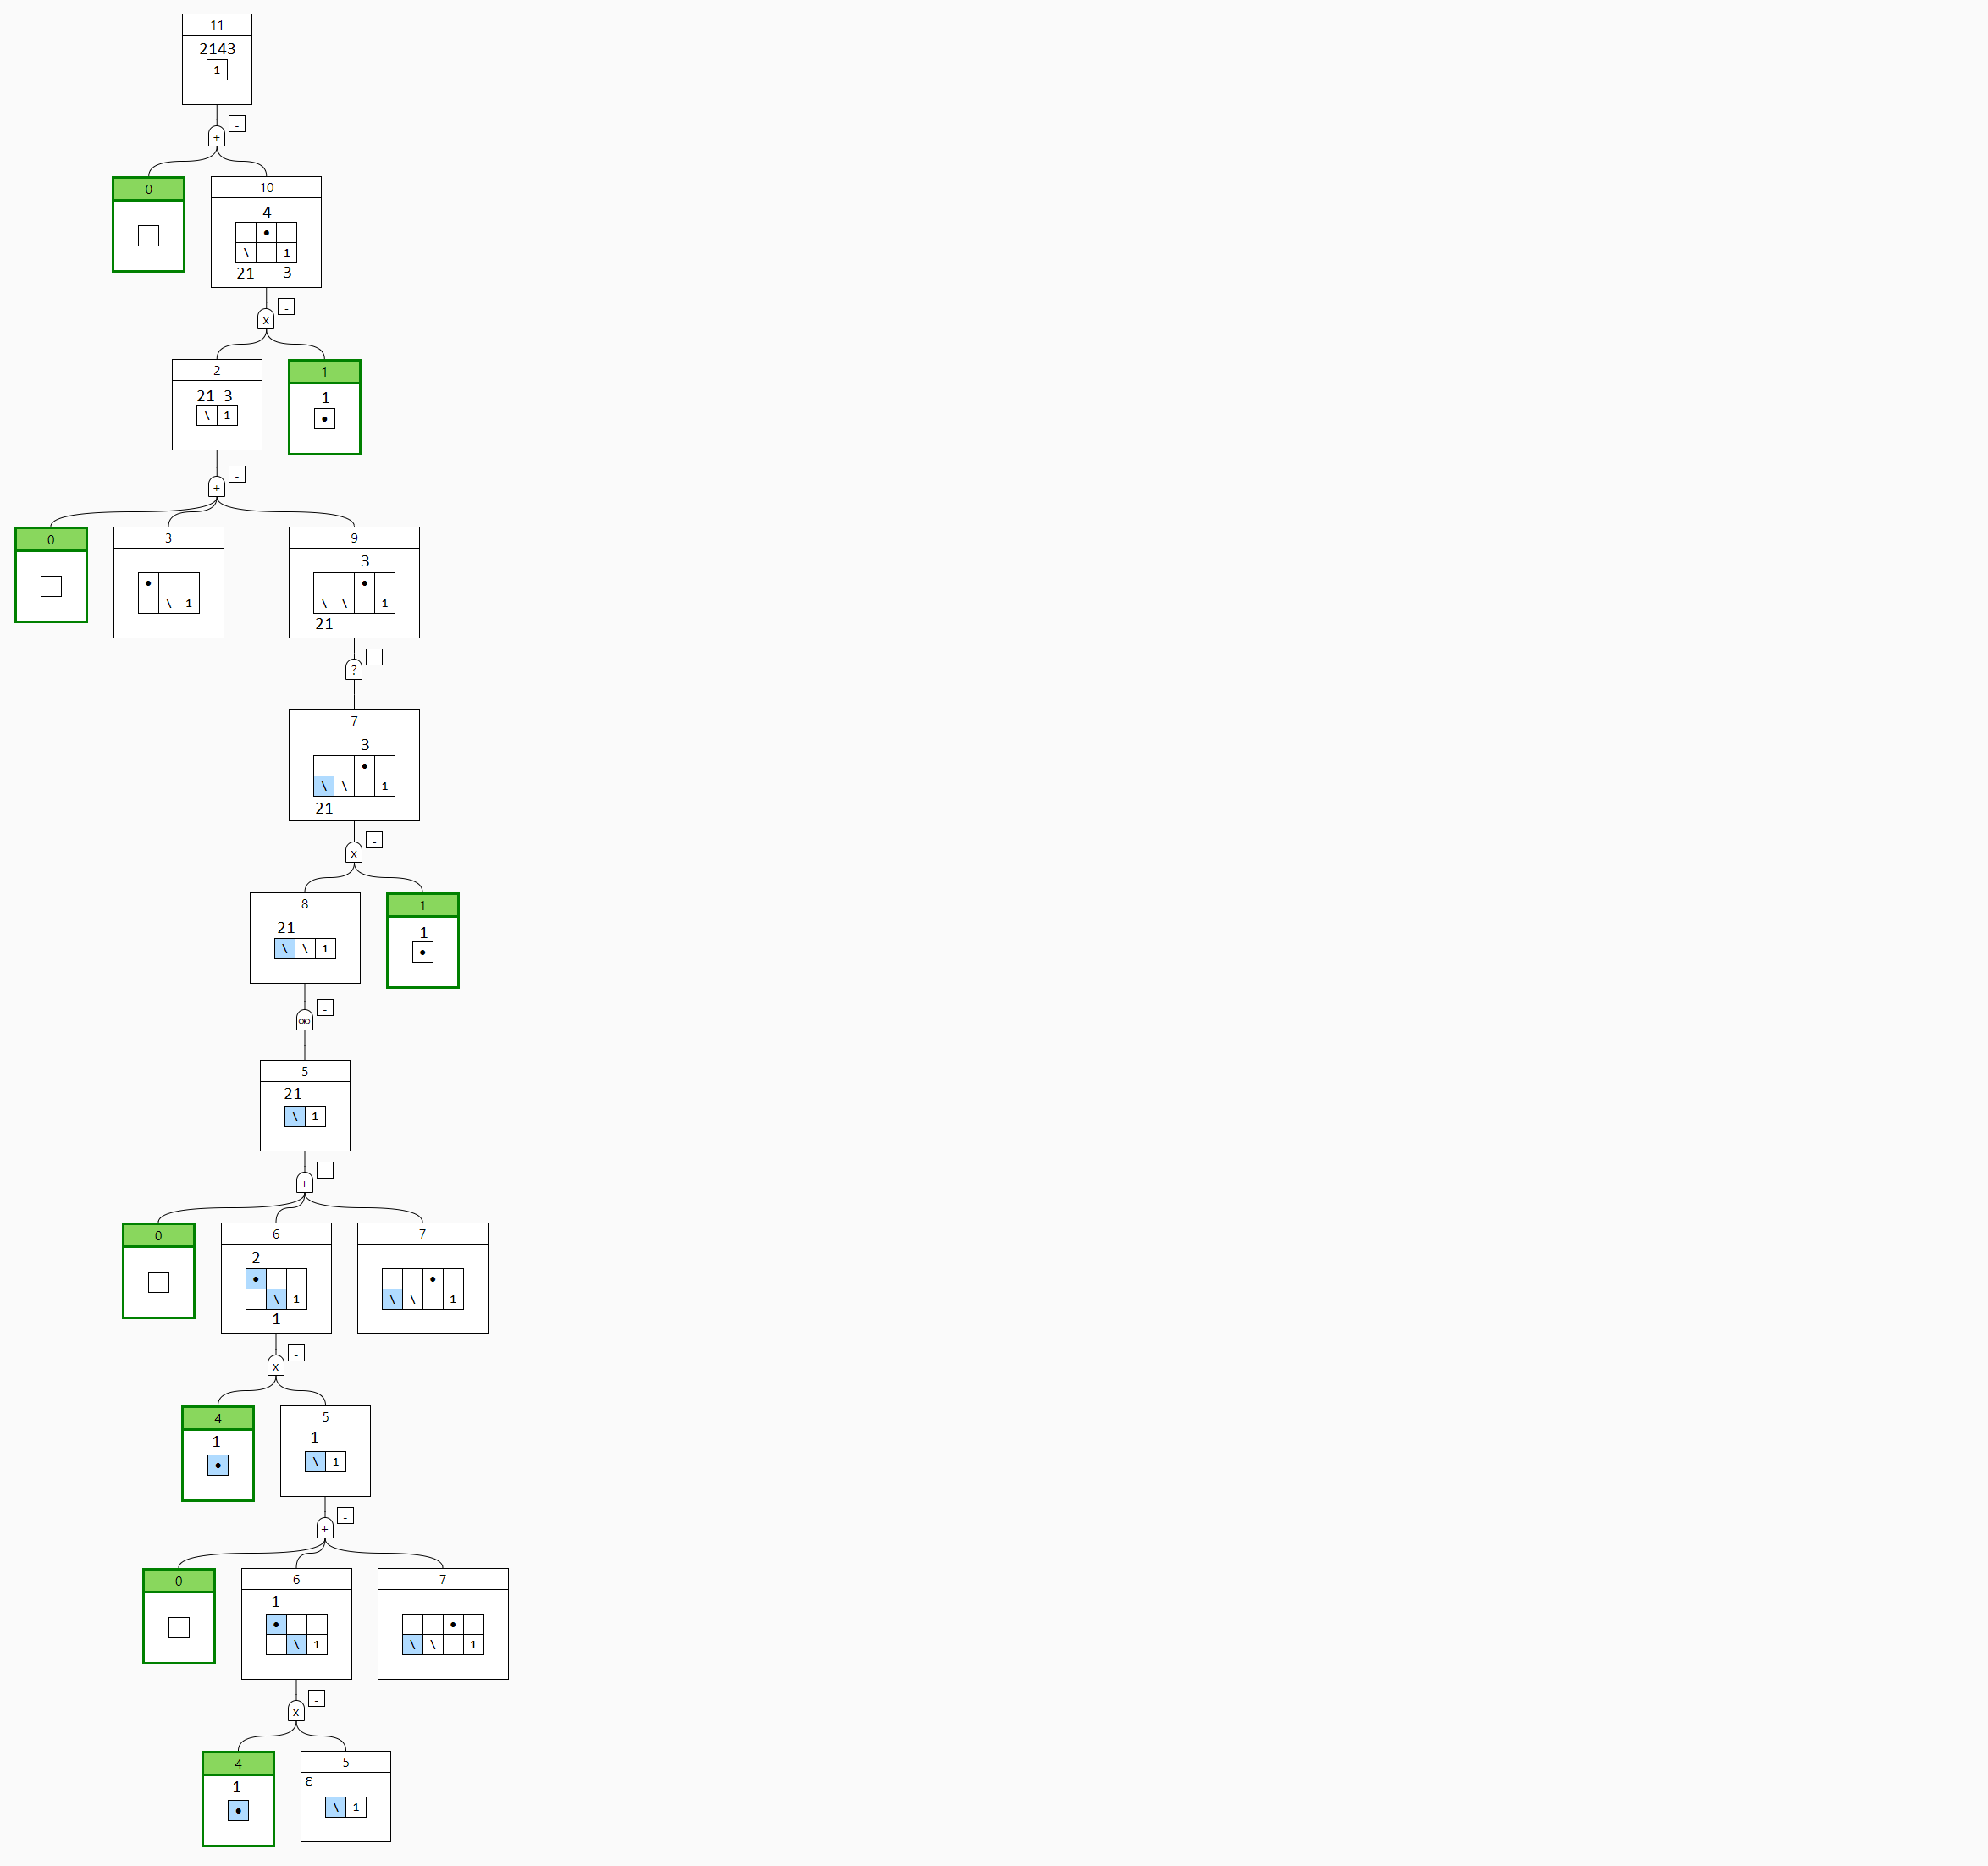
\includegraphics[scale=0.12]{graphics/parse_trees_01.png}};
        }
        \only<2>{%
            \tikz [remember picture,overlay] \node at ([yshift=-.25cm,xshift=0cm]current page.center) {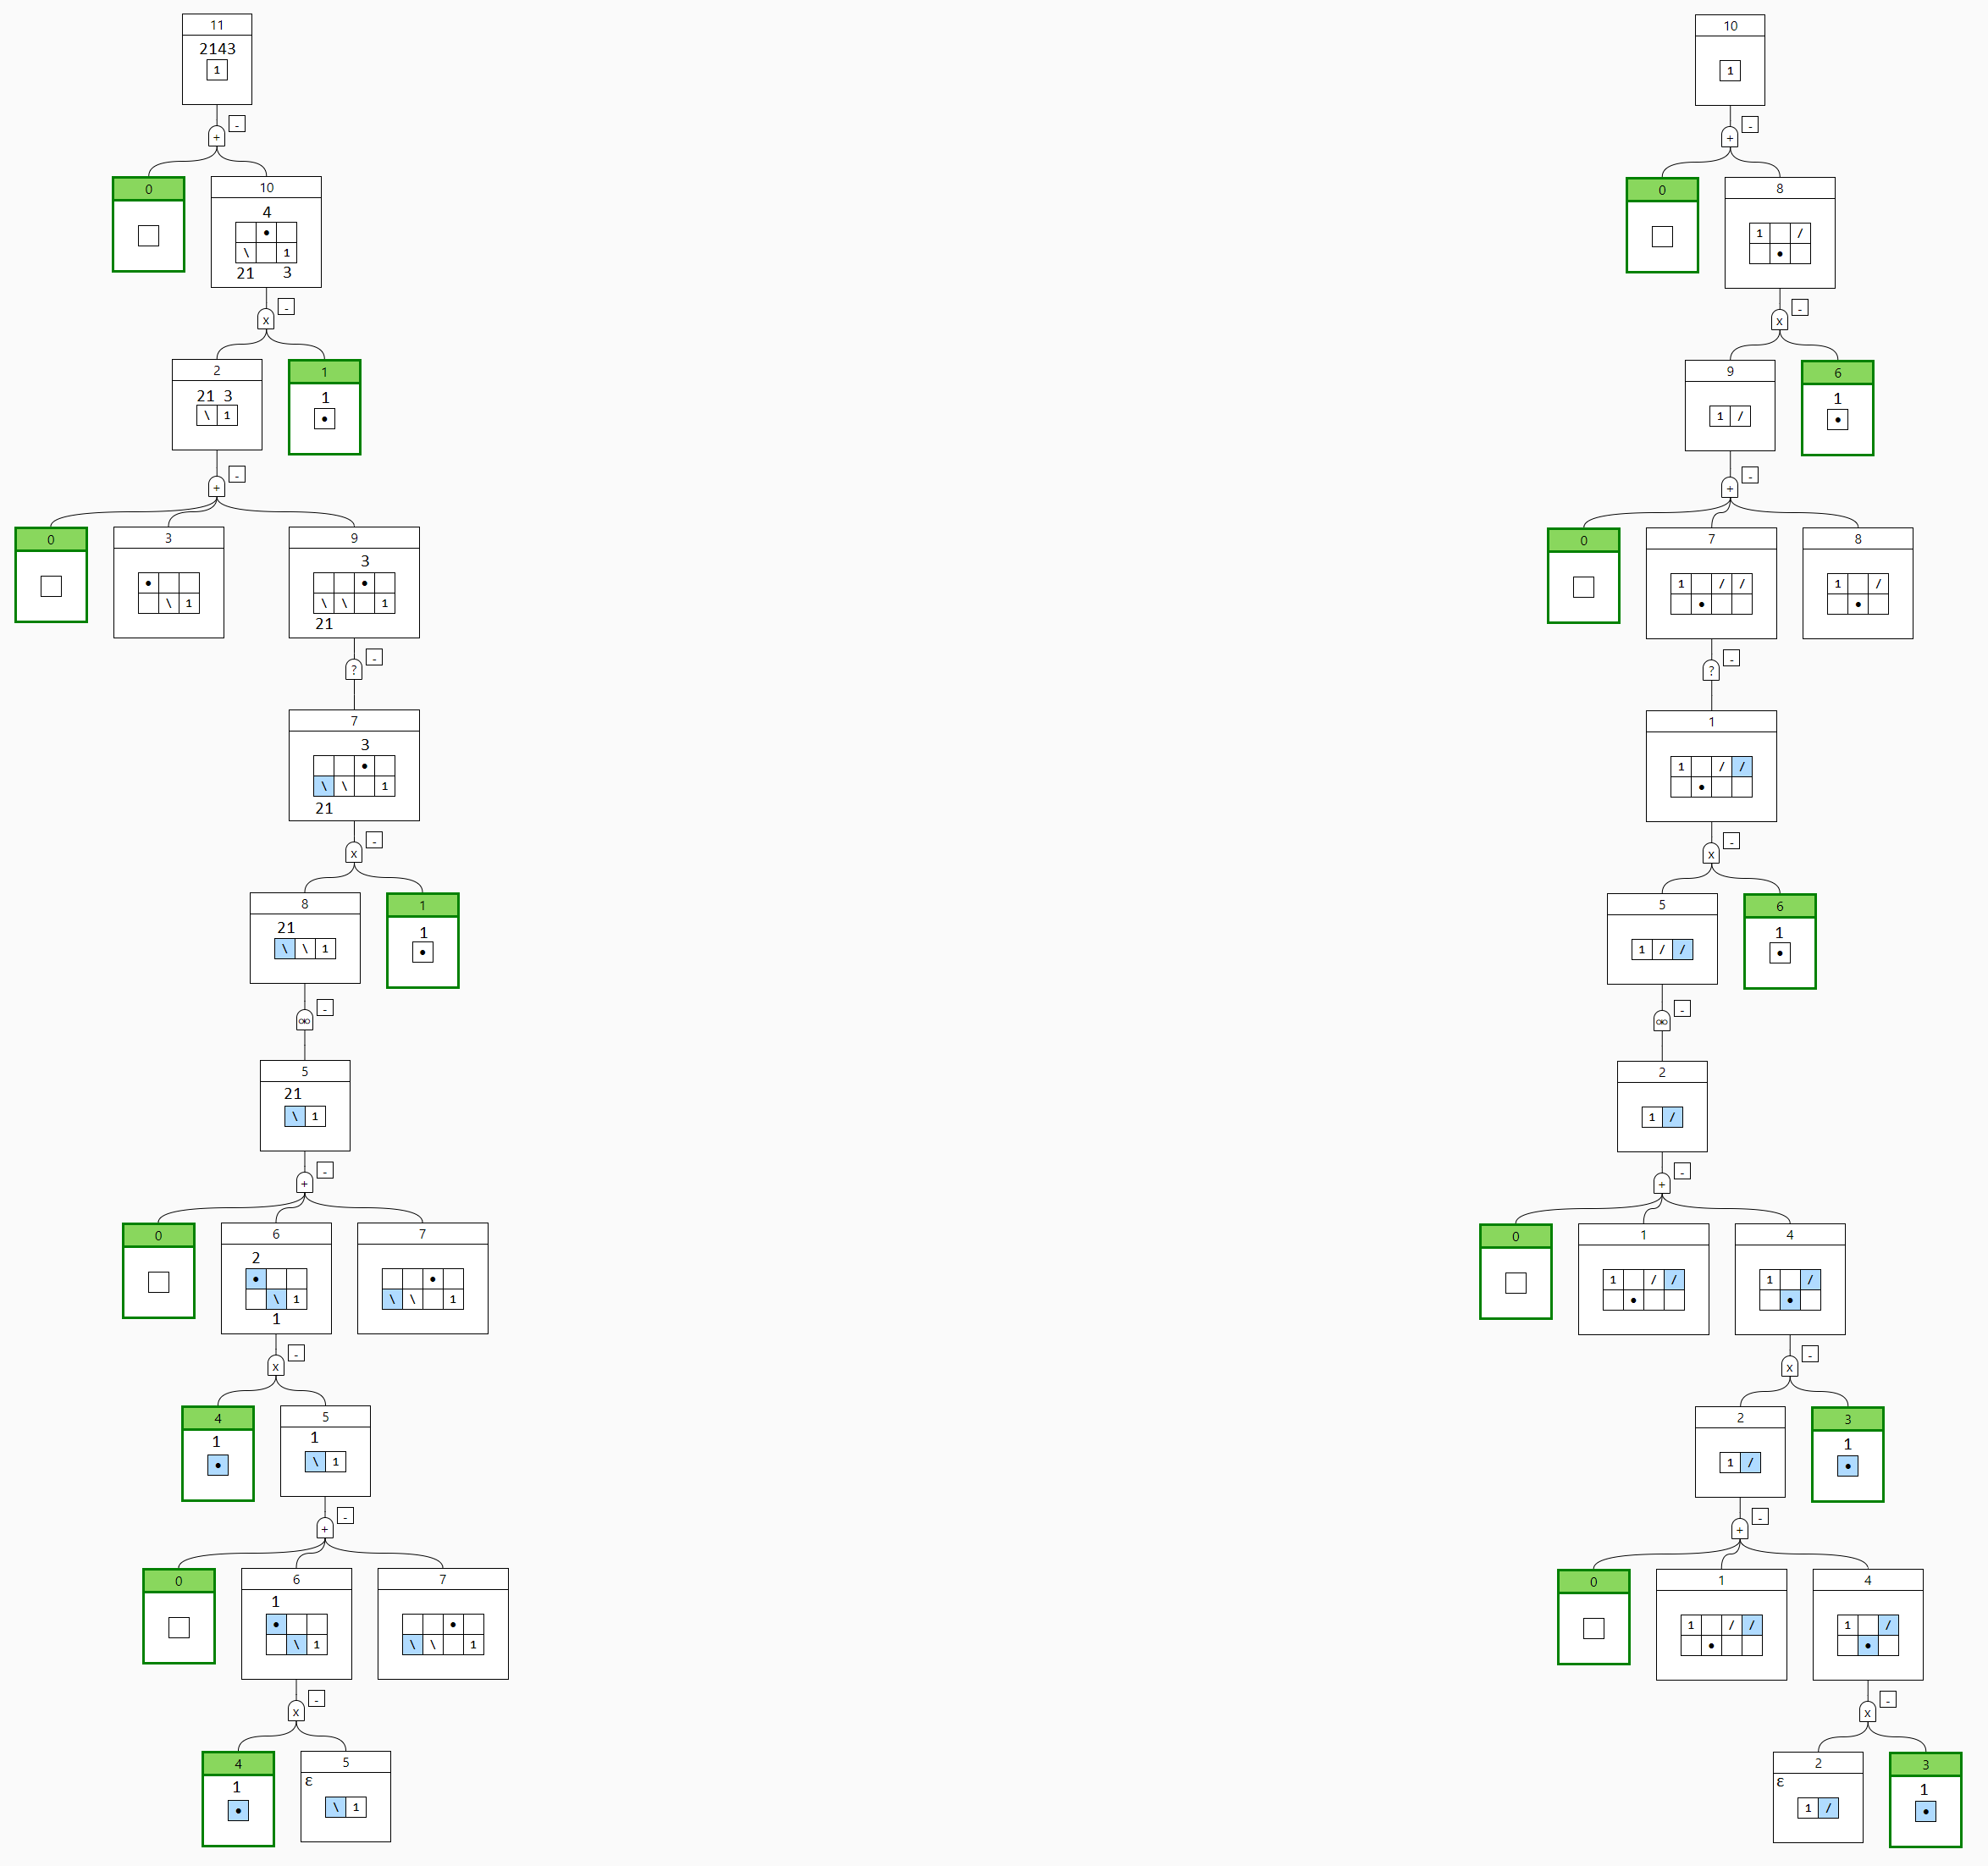
\includegraphics[scale=0.12]{graphics/parse_trees_02.png}};
        }
        \only<3>{%
            \tikz [remember picture,overlay] \node at ([yshift=-.25cm,xshift=0cm]current page.center) {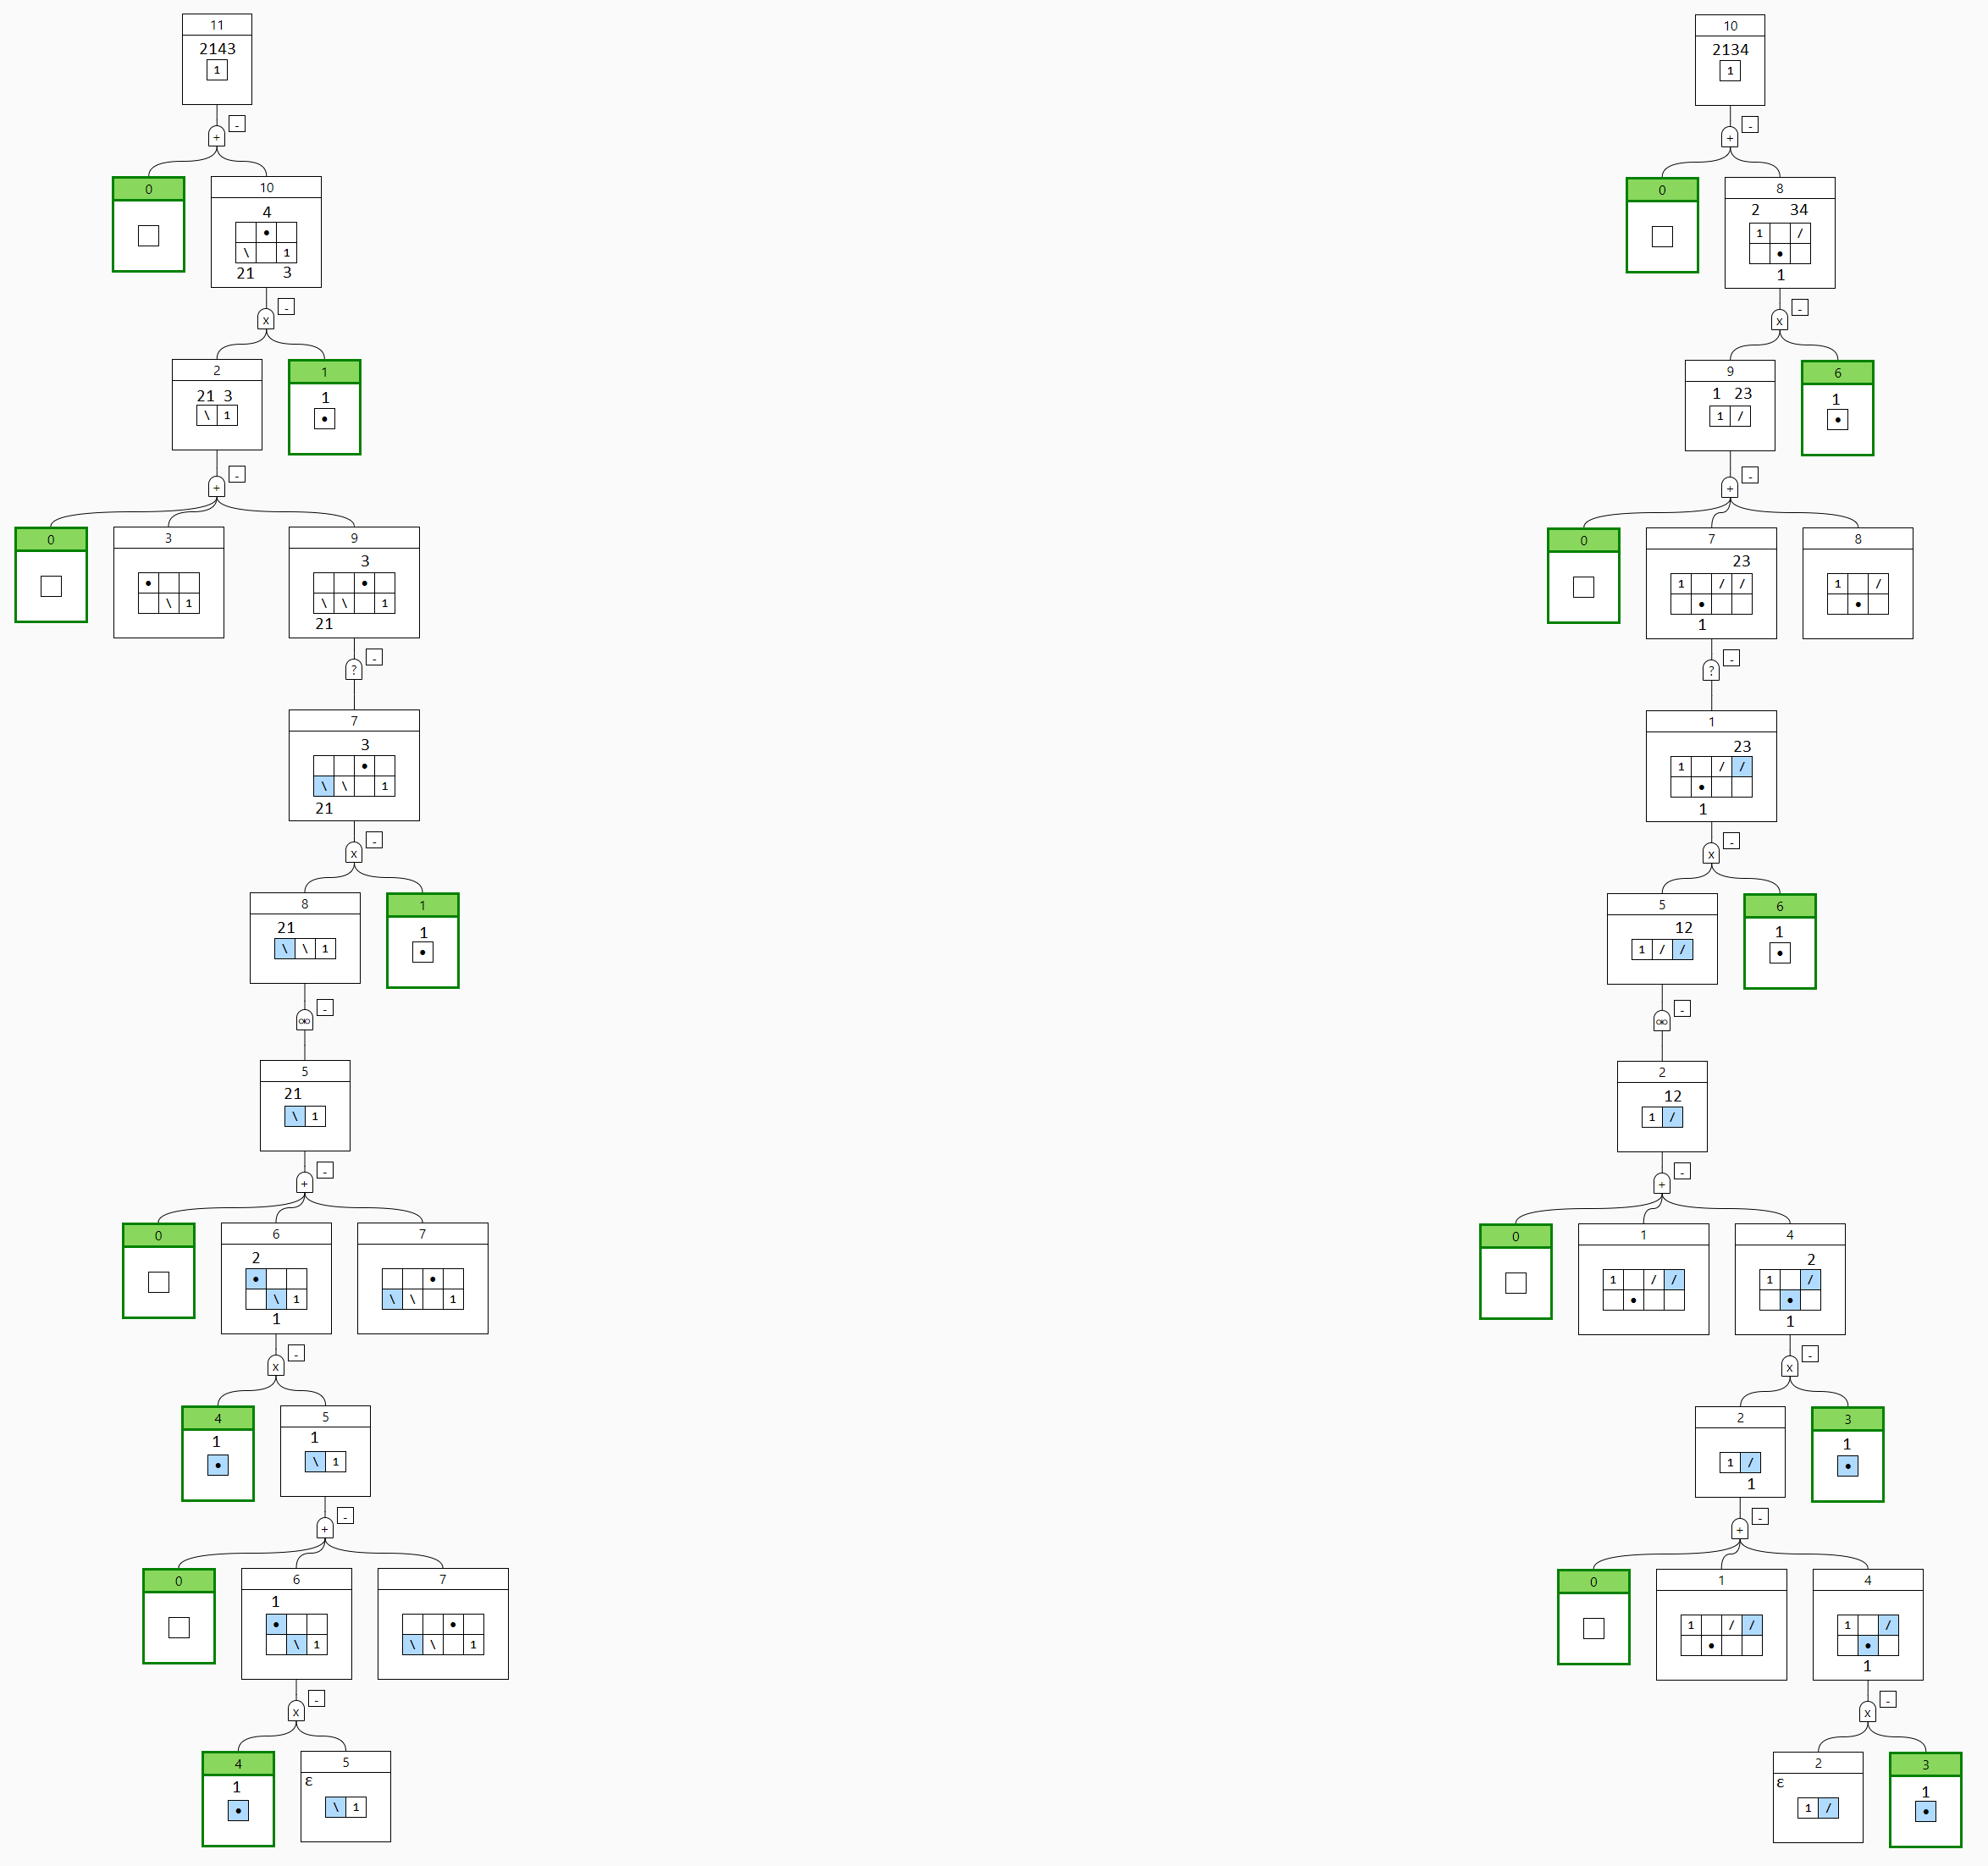
\includegraphics[scale=0.12]{graphics/parse_trees_03.png}};
        }
        \only<4>{%
            \tikz [remember picture,overlay] \node at ([yshift=-.25cm,xshift=0cm]current page.center) {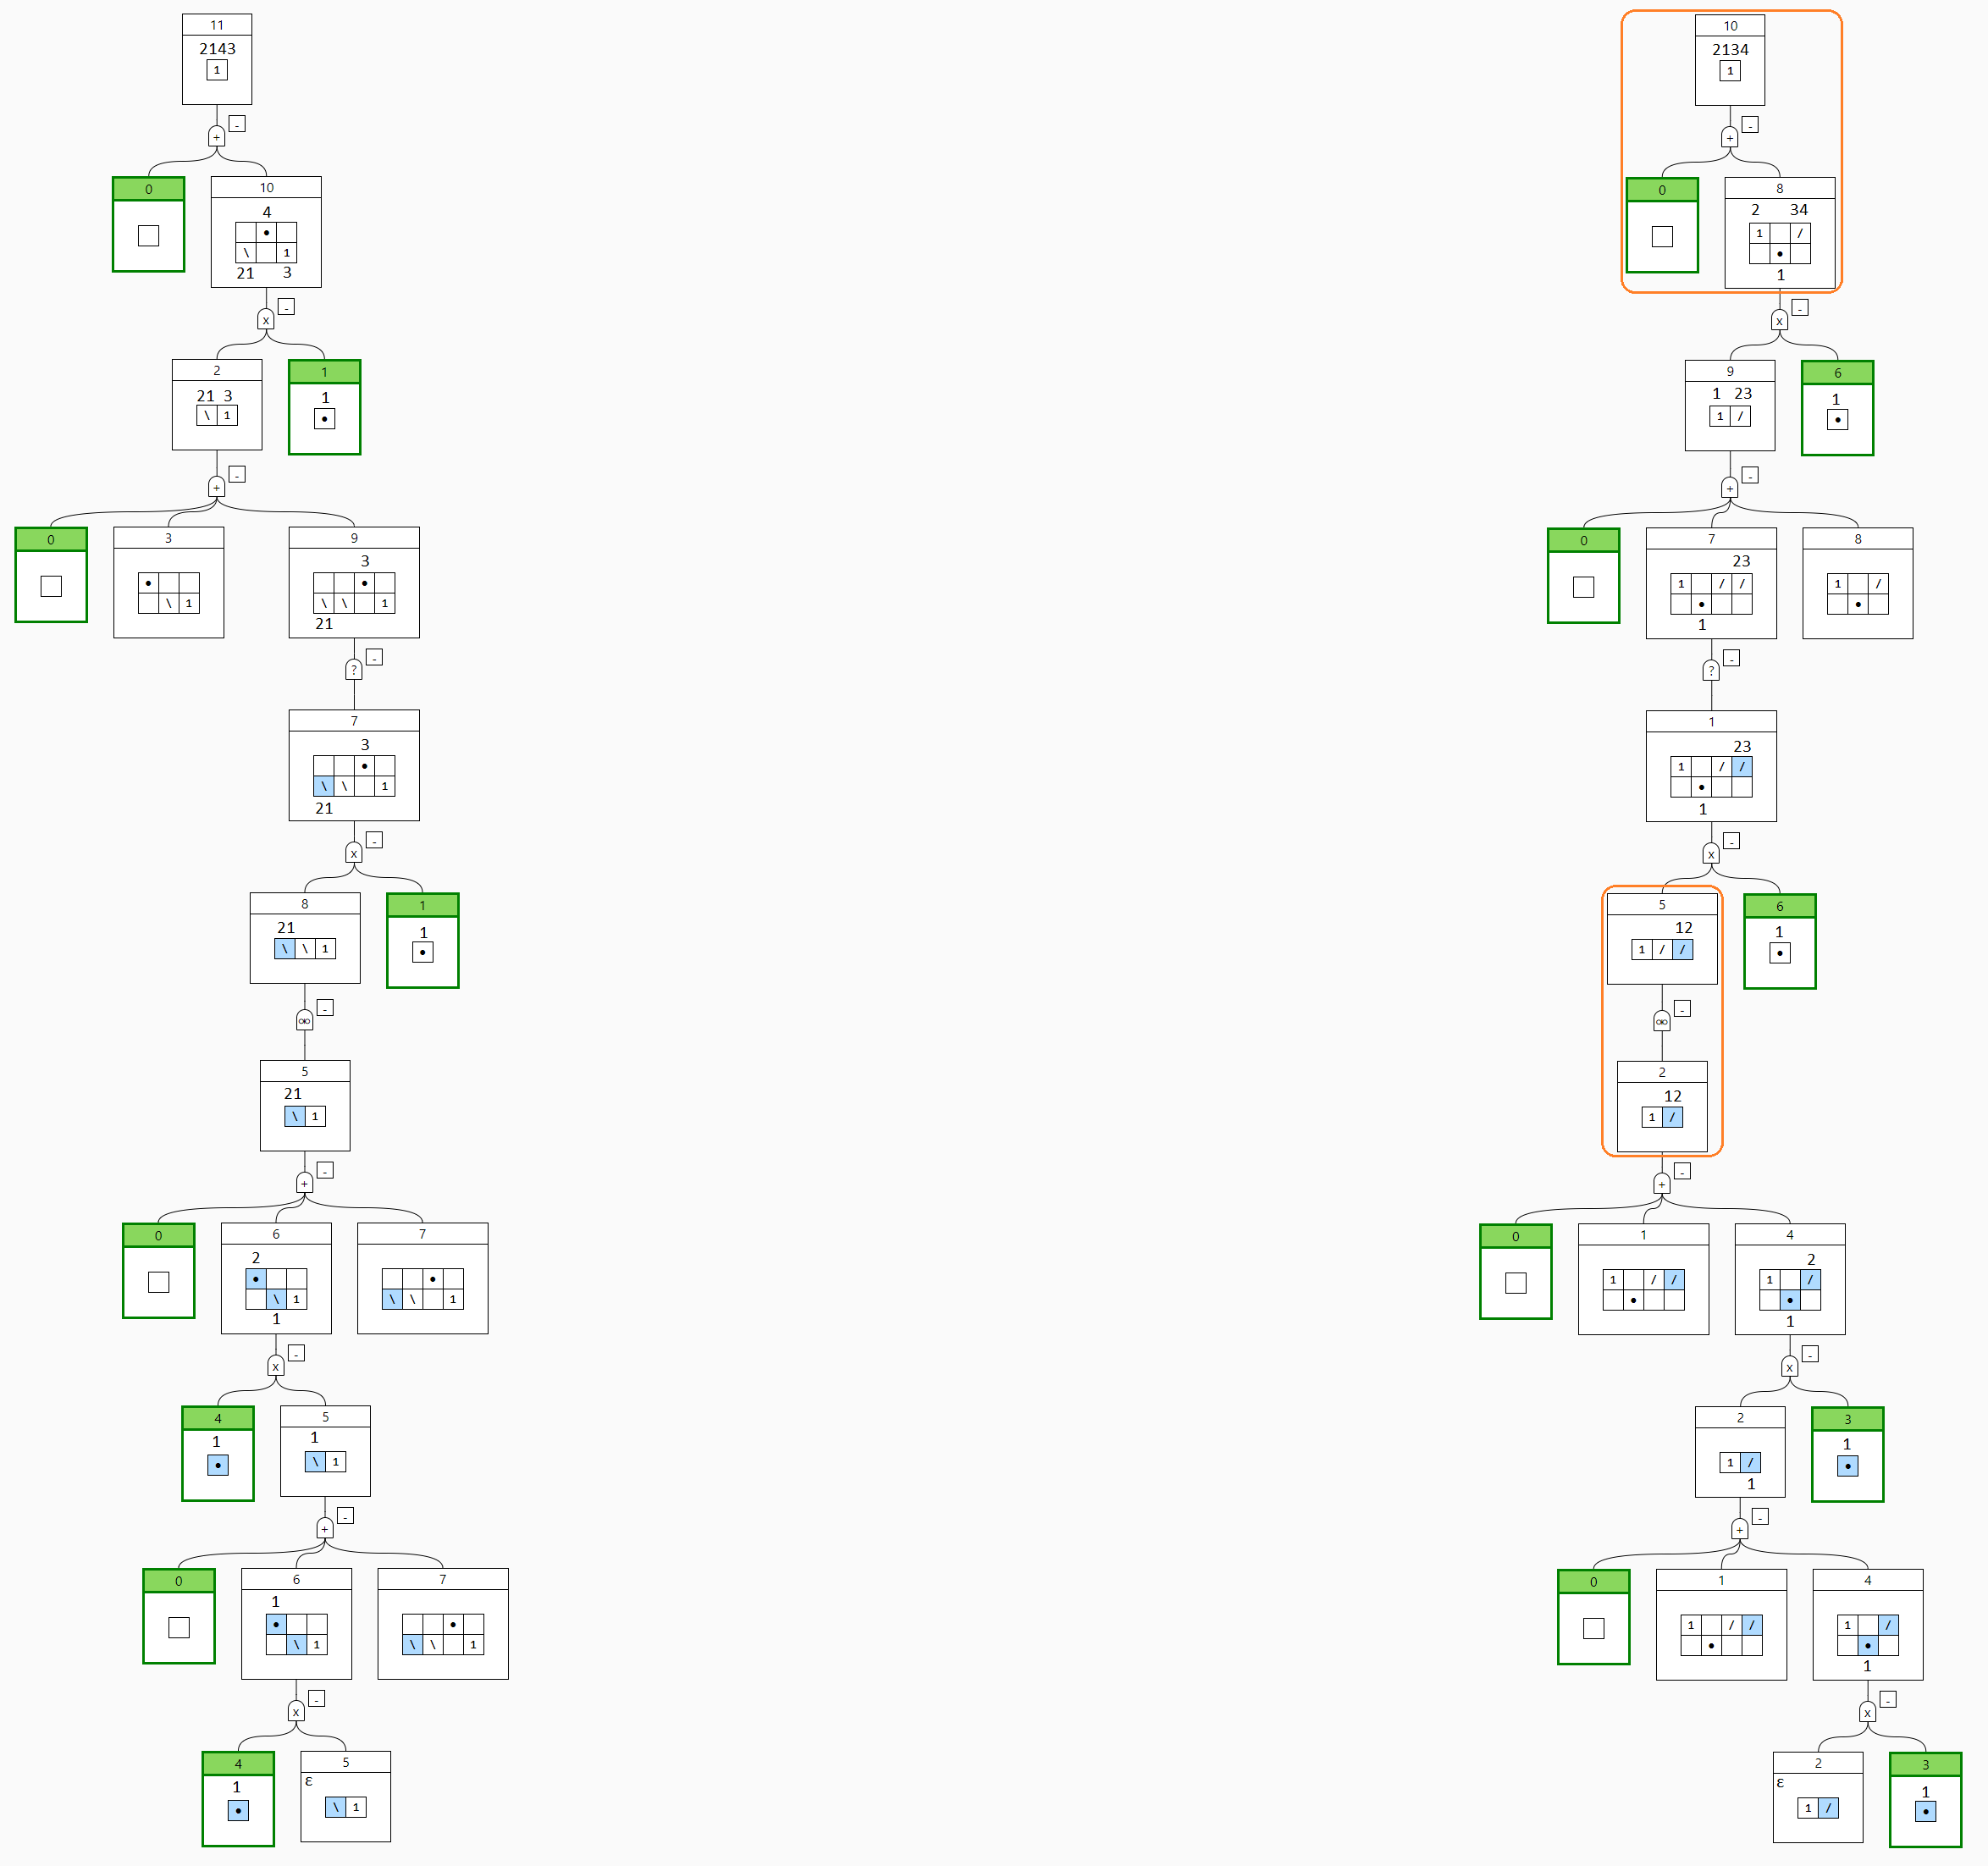
\includegraphics[scale=0.12]{graphics/parse_trees_04.png}};
        }
        %\onslide<2->
    \end{figure}
\end{frame}

% Backward

\begin{frame}{Parallel bijection - An example for $\Av{123}$ and $\Av{132}$}
    \begin{figure}
        \centering
        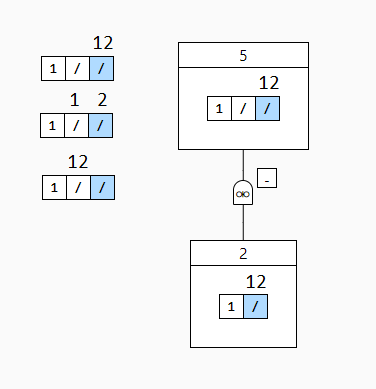
\includegraphics[scale=0.4]{graphics/fus_back.png}
        \caption{Backward step for fusion.}
    \end{figure}
\end{frame}
\begin{frame}{Parallel bijection - An example for $\Av{123}$ and $\Av{132}$}
    Final step
    \begin{figure}
        \centering
        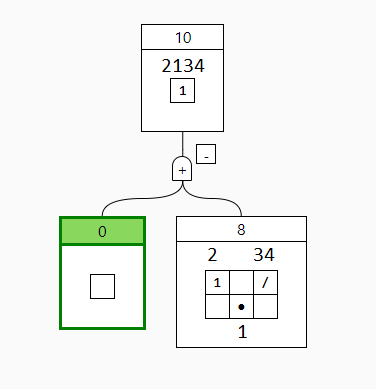
\includegraphics[scale=0.4]{graphics/final_parse.png}
        \caption{Final step.}
    \end{figure}
\end{frame}